\documentclass[lettersize,journal]{IEEEtran}
\usepackage[T1]{fontenc}
\usepackage{amsmath,amsfonts,amssymb}
\usepackage{array}
\usepackage{booktabs}
\usepackage{multirow}
\usepackage{graphicx}
\usepackage{textcomp}
\usepackage{stfloats}
\usepackage{url}
\usepackage{cite}
\usepackage{xcolor}
\usepackage{tikz}
\usetikzlibrary{positioning,arrows.meta,fit,calc,backgrounds}
\usepackage[hidelinks]{hyperref}
\graphicspath{{figures/}}
\hyphenation{Efficient-Net SIPaKMeD NHANES question-naire}

% ---------------------------------------------------------------- float placement
\renewcommand{\topfraction}{0.92}
\renewcommand{\bottomfraction}{0.70}
\renewcommand{\textfraction}{0.06}
\renewcommand{\floatpagefraction}{0.70}
\renewcommand{\dbltopfraction}{0.92}
\renewcommand{\dblfloatpagefraction}{0.70}
\setcounter{topnumber}{3}
\setcounter{bottomnumber}{2}
\setcounter{totalnumber}{5}
\setcounter{dbltopnumber}{3}

% ---------------------------------------------------------------- notation
\newcommand{\logit}{\operatorname{logit}}
\newcommand{\pimg}{p_{\mathrm{img}}}
\newcommand{\ptab}{p_{\mathrm{tab}}}
\newcommand{\piimg}{\pi_{\mathrm{img}}}
\newcommand{\pitab}{\pi_{\mathrm{tab}}}
% seed repeats and distillation ablation (filled from results/variants/)
\newcommand{\SeedStudent}{$0.946\pm0.016$}
\newcommand{\SeedTeacher}{$0.938\pm0.032$}
\newcommand{\KDnone}{0.955}
\newcommand{\KDprob}{0.958}
\newcommand{\KDlogit}{0.950}
\newcommand{\KDlogitTT}{0.960}

\tikzset{
  box/.style={draw, rounded corners=2pt, align=center, font=\footnotesize, inner sep=3pt, minimum height=8mm, fill=white},
  data/.style={box, fill=gray!10},
  model/.style={box, line width=0.9pt},
  op/.style={box, dashed},
  arr/.style={-{Stealth[length=2mm]}, line width=0.6pt},
  var/.style={draw, circle, inner sep=1.4pt, font=\footnotesize, minimum size=9mm, fill=white},
  vtag/.style={font=\scriptsize\bfseries, color=red!70!black, fill=white, inner sep=1pt},
}

\begin{document}

\title{Fusing Unpaired Cytology and Questionnaire Experts for Cervical Screening: A Calibrated Rule and Its Region of Validity}

\author{Author One, Author Two, Author Three, and Author Four
\thanks{Manuscript received XX; revised XX. (Corresponding author: Author One.)}
\thanks{The authors are with MUICT RAS (affiliation to be completed; e-mail: corresponding@author.org).}
\thanks{This work was supported by [funding source and grant number to be completed].}
\thanks{The authors declare no conflicts of interest.}}

\markboth{IEEE Journal of Biomedical and Health Informatics}%
{Fusing Unpaired Cytology and Questionnaire Experts for Cervical Screening}

\maketitle

\begin{abstract}
Cervical screening weighs cell morphology together with infection risk, yet public data sets never pair a cytology image with a risk questionnaire from the same woman, so a joint model cannot be trained. We study a decision-level rule that fuses two independently trained experts without paired data: it removes each expert's training prevalence, converts questionnaire-estimated infection risk into a pre-test probability of abnormal cytology through an epidemiological link estimated from 812,598 co-tests, and treats the image as a likelihood ratio; split-conformal prediction lets the system abstain. A distilled EfficientNet-B0 cytology expert reached 96.4\% accuracy on held-out cells and 95.8\% when whole slides were held out, but only 0.641 area under the curve on an external collection, rising to 0.805 once a cell type absent from training was excluded. A questionnaire expert built from 12,634 women in seven national survey cycles reached 0.694 area under the curve under nested model selection and 0.713 under survey weighting. On semi-synthetic cohorts that pair real held-out records, the unpaired rule matched a model trained on paired patients whenever its assumptions held, and equalled a model given about two hundred paired patients. We then broke those assumptions in turn. The rule tolerates a misspecified link, subgroup-varying links and unknown miscalibration, but loses its advantage once residual dependence between the modalities exceeds about 0.2, and prevalence re-anchoring cannot repair the miscalibration that domain shift causes. We therefore report a calibrated any-modality screening output together with an explicitly mapped region of validity.
\end{abstract}

\begin{IEEEkeywords}
Cervical cancer screening, multimodal fusion, missing modality, probability calibration, prior shift, knowledge distillation, conformal prediction, human papillomavirus, external validation, explainable AI.
\end{IEEEkeywords}

%% =====================================================================
\section{Introduction}
\IEEEPARstart{C}{ervical} cancer remains one of the most common cancers in women worldwide, with most deaths occurring where routine screening and timely diagnosis are limited \cite{WHO_cervical_cancer}. Persistent infection with a high-risk human papillomavirus (HPV) genotype is a necessary cause of the disease \cite{walboomers1999hpv}, and screening programmes therefore combine two complementary views: HPV testing, which measures infection, and cytology, which measures the cellular changes the infection produces \cite{WHO_screening_guideline}. A decision-support tool that weighs a woman's infection risk together with the appearance of her cells would mirror that reasoning.

Artificial intelligence already performs strongly on each view separately. Convolutional networks classify Pap-smear cells with high in-distribution accuracy \cite{zhang2017deeppap,tan2024cervical,youneszade2023deep}, and machine-learning models estimate risk from questionnaire variables \cite{fernandes2017cervical,sun2022stacking,chadaga2022predicting}. Multimodal models combining images with clinical variables have shown gains in related cervical tasks \cite{das2026topoticerv,wang2025cervipro,sha2024cervifusionnet}, and multimodal biomedical AI is an active direction more broadly \cite{acosta2022multimodal,baltrusaitis2019multimodal}.

Two obstacles block such a tool when only public data are available. First, the modalities are \emph{unpaired}: cytology collections such as SIPaKMeD \cite{plissiti2018sipakmed} and Herlev \cite{jantzen2005herlev} carry no patient-level risk information, while risk-factor surveys such as the U.S. National Health and Nutrition Examination Survey (NHANES) \cite{nhanes} carry no images. Joint-training and missing-modality methods \cite{havaei2016hemis,yao2024drfuse,wu2026deep} still need patients observed in more than one modality. Second, the two experts answer \emph{different questions} under \emph{different prevalences}: one predicts infection, the other cellular abnormality, and each was trained on a class mix unlike that of a screening clinic.

A decision-level rule can bridge both gaps. Removing an expert's training prior and re-anchoring it to the deployment prevalence is standard under label shift \cite{saerens2002adjusting,lipton2018labelshift}; converting infection risk into a pre-test probability of abnormal cytology requires only two epidemiological rates; and combining the two as prior odds times a likelihood ratio is the textbook diagnostic calculation. The resulting rule needs no paired data and no retraining. Its weakness is that it is exactly as good as its assumptions, and those assumptions -- conditional independence of the two records given the cytological state, calibrated experts, and a known link -- are not verifiable from unpaired data.

This paper therefore does two things. It builds and reports the two experts under leakage-aware protocols, including external validation of the image expert. And it treats the fusion rule as a hypothesis to be attacked rather than demonstrated: we estimate the epidemiological link from a large screening cohort rather than assuming it, evaluate the rule on semi-synthetic cohorts assembled from real held-out records, and then break each assumption in turn to find where the rule stops working.

The contributions are:
\begin{enumerate}
\item \emph{Two calibrated experts, honestly evaluated.} A distilled cytology classifier that matches its teacher with four times fewer parameters, reported on a fixed test set, under a slide-grouped protocol, and on an external data set; and a questionnaire expert on 12,634 NHANES participants with in-fold preprocessing, one-hot encoding of nominal items, missingness indicators, nested model selection, survey-weighted and temporal sensitivity analyses, and subgroup calibration.
\item \emph{A link estimated, not assumed.} The infection-to-cytology bridge is derived from the full co-test cross-tabulation of 812,598 screening co-tests, giving an odds ratio of 17.9 (95\% CI 17.5--18.3) instead of a swept hyper-parameter.
\item \emph{A region of validity.} Six controlled violations of the fusion's assumptions, showing that it tolerates link misspecification, subgroup-varying links and unknown miscalibration, but loses its advantage beyond a residual dependence of about 0.2, and cannot repair domain-shift miscalibration.
\item \emph{A price in paired data.} The unpaired rule is shown to be worth roughly two hundred paired patients, quantifying what one gives up by not having them.
\item \emph{Negative and boundary results reported in full}, including a case under real domain shift in which naive averaging outperforms the principled rule.
\end{enumerate}

Fig.~\ref{fig:framework} summarises the system and Fig.~\ref{fig:dag} states the assumptions it rests on.

\begin{figure*}[t]
\centering
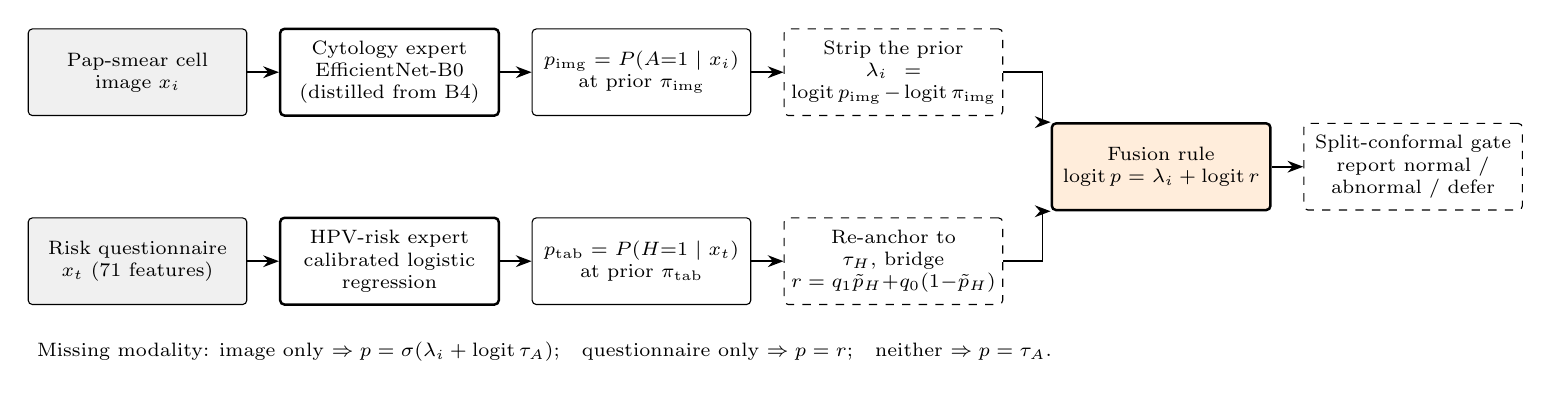
\begin{tikzpicture}[x=1mm, y=1mm, font=\footnotesize]
  \tikzset{
    fbox/.style={draw, rounded corners=1.5pt, align=center, font=\scriptsize, inner sep=2.5pt,
                 text width=26mm, minimum height=11mm, fill=white},
    fdata/.style={fbox, fill=gray!12},
    fmodel/.style={fbox, line width=0.9pt},
    fop/.style={fbox, dashed},
  }
  % top row: the cytology path; bottom row: the questionnaire path
  \node[fdata]  (img) at (  0, 12) {Pap-smear cell\\image $x_i$};
  \node[fmodel] (ce)  at ( 32, 12) {Cytology expert\\EfficientNet-B0\\(distilled from B4)};
  \node[fbox]   (pi)  at ( 64, 12) {$\pimg=P(A{=}1\mid x_i)$\\at prior $\piimg$};
  \node[fop]    (lr)  at ( 96, 12) {Strip the prior\\$\lambda_i=\logit\pimg-\logit\piimg$};
  \node[fdata]  (tab) at (  0,-12) {Risk questionnaire\\$x_t$ (71 features)};
  \node[fmodel] (he)  at ( 32,-12) {HPV-risk expert\\calibrated logistic\\regression};
  \node[fbox]   (pt)  at ( 64,-12) {$\ptab=P(H{=}1\mid x_t)$\\at prior $\pitab$};
  \node[fop]    (an)  at ( 96,-12) {Re-anchor to $\tau_H$, bridge\\$r=q_1\tilde p_H+q_0(1-\tilde p_H)$};
  \node[fmodel, fill=orange!14] (fu) at (130, 0) {Fusion rule\\$\logit p=\lambda_i+\logit r$};
  \node[fop]    (cp) at (162, 0) {Split-conformal gate\\report normal / abnormal / defer};
  \foreach \a/\b in {img/ce, ce/pi, pi/lr, tab/he, he/pt, pt/an} {\draw[arr] (\a) -- (\b);}
  \draw[arr] (lr.east) -- ++(5,0) |- (fu.north west);
  \draw[arr] (an.east) -- ++(5,0) |- (fu.south west);
  \draw[arr] (fu) -- (cp);
  \node[font=\scriptsize, anchor=north west] at (-14,-21)
    {Missing modality: image only $\Rightarrow p=\sigma(\lambda_i+\logit\tau_A)$;\quad
     questionnaire only $\Rightarrow p=r$;\quad neither $\Rightarrow p=\tau_A$.};
\end{tikzpicture}
\caption{Overview of the system. Two experts are trained on separate, unpaired data sets and are never retrained jointly. The cytology expert predicts cellular abnormality $A$; the questionnaire expert predicts high-risk HPV infection $H$. The rule removes each expert's training prior, maps infection risk to a pre-test probability of abnormal cytology through the link probabilities $q_1=P(A{=}1\mid H{=}1)=0.364$ and $q_0=P(A{=}1\mid H{=}0)=0.031$ estimated in Section~\ref{sec:link}, and adds the image evidence as a log-likelihood ratio. A split-conformal gate defers cases whose prediction set is not a single class. The assumptions under which this is exact are stated in Fig.~\ref{fig:dag}.}
\label{fig:framework}
\end{figure*}
\section{Related Work}

\subsection{Clinical risk factors and machine-learning risk prediction}
Before deep learning, cervical cancer prediction relied mainly on traditional machine-learning algorithms trained on structured clinical information and patient risk factors. Early studies compared numerous supervised learners, and ensembles of several classifiers generally outperformed individual models, with tree-based methods achieving high accuracy on the UCI Cervical Cancer Risk Factors data set \cite{fernandes2017cervical}. Imputation strategies ranging from mean substitution to $k$-nearest-neighbour and support-vector-machine imputation have been used to reconstruct missing clinical information before training \cite{karamti2023improvingpr,munshi2024novel}. Severe class imbalance is commonly addressed with oversampling such as SMOTE, SMOTE-Tomek links, ADASYN and random oversampling, often combined with outlier detection \cite{ijaz2020data}, and voting, boosting and stacking ensembles have been investigated to improve performance \cite{sun2022stacking,chadaga2022predicting}. When oversampling or imputation is fitted before the data are split, however, synthetic or imputed information leaks into the evaluation folds; we therefore fit every preprocessing step inside the cross-validation loop and use class weighting instead of synthetic oversampling.

\subsection{Deep learning for cervical cytology}
Deep learning has advanced cervical cancer diagnosis by learning features directly from images. DeepPap was among the first studies to apply deep convolutional networks and transfer learning to cervical cell classification, showing that ImageNet-pretrained representations adapt effectively to cytology despite limited annotated data \cite{zhang2017deeppap}. A comparison of thirteen pretrained architectures found DenseNet-201 to perform best on the Herlev data set \cite{tan2024cervical}. Whole-slide frameworks combine patch-level networks with slide-level aggregation and have been evaluated on independent private cohorts \cite{yan2025deep}, and Swin-Transformer ensembles have been applied to colposcopy images \cite{himabindu2025swin}. Reviews highlight persistent challenges: limited data-set diversity, class imbalance, lack of external validation and difficult clinical translation \cite{vallescoral2026review,youneszade2023deep}.

\subsection{Foundation models}
These limitations have motivated pathology foundation models that learn transferable representations from very large collections. UniCAS is a cervical cytology foundation model pretrained with self-supervision on more than 48,000 whole-slide images and evaluated on screening, candidiasis detection and subtype diagnosis \cite{jiang2026unicas}. General-purpose pathology models such as UNI \cite{chen2024uni}, the vision-language model CONCH \cite{lu2024visual}, the multimodal slide-level model TITAN \cite{ding2025titan} and the gigapixel model Prov-GigaPath \cite{xu2024provgigapath} provide representations that may benefit cervical pathology when labelled data are scarce.

\subsection{Multimodal learning for cervical cancer}
Clinical decisions also draw on information outside the image, such as age, HPV status, smoking history, parity and previous findings. TopotiCerv integrates acetowhite colposcopic images with clinical findings for lesion classification \cite{das2026topoticerv}; Wang \emph{et al.} combined pre- and post-treatment CT, radiomic features and clinical variables to predict disease-free survival after radiotherapy \cite{wang2025cervipro}; CerviFusionNet fuses original, acetic-acid and iodine colposcopic images through a hybrid CNN--Transformer--GRU network \cite{sha2024cervifusionnet}; radiomic and deep features have been combined for lesion detection with external validation \cite{niu2025hybridfeatu}; and graph neural networks have fused segmented regions within colposcopy images \cite{chatterjee2025multi}. Incomplete patient information is a practical challenge, addressed through feature completion, modality hallucination, distillation and modality-invariant representations \cite{wu2026deep,havaei2016hemis,yao2024drfuse}. All of these approaches learn cross-modal interactions from patients observed in more than one modality; none addresses the case in which the modalities come from entirely disjoint populations.

\subsection{Data-set heterogeneity and label harmonisation}
Public cytology collections, including Herlev \cite{jantzen2005herlev}, SIPaKMeD \cite{plissiti2018sipakmed}, CRIC \cite{rezende2021cric}, APACC \cite{kupas2024apacc} and HiCervix \cite{cai2024hicervix}, differ in acquisition, staining, magnification, segmentation, class distributions and annotation schemes \cite{coskun2026robust}, and newer liquid-based cytology sets add further diversity \cite{hussain2020liquidbased}. The Bethesda System provides a clinically established vocabulary for cytology reporting that supports medically justified harmonisation of heterogeneous labels \cite{solomon2002bethesda,nayar2015bethesda}; we use it to collapse the five SIPaKMeD cell types into the binary normal/abnormal decision that the fusion consumes. Large-scale validation, such as the multicentre retrospective, prospective and randomised evaluation reported by Wang \emph{et al.} \cite{wang2024aiccs}, remains the benchmark for trustworthy screening AI. Explainability methods, including SHAP feature attribution, LIME and Grad-CAM localisation, are increasingly reported alongside performance \cite{vallescoral2026review}.

\subsection{Decision-level fusion, calibration and uncertainty}
Classifier-combination rules such as the product and sum rules \cite{kittler1998combining} assume experts that output posteriors for the \emph{same} label under the \emph{same} prior. When class priors differ between training and deployment, posteriors can be corrected by Bayes' rule without retraining \cite{saerens2002adjusting,lipton2018labelshift}. Modern networks are frequently miscalibrated \cite{guo2017calibration}, and Platt scaling \cite{platt1999probabilistic} and isotonic regression \cite{zadrozny2002transforming} are standard remedies. Conformal prediction offers distribution-free coverage guarantees \cite{vovk2005algorithmic,angelopoulos2023conformal} and has recently been validated for cervical atypia classification \cite{hagos2026conformal}; cytologist-in-the-loop systems show the clinical value of deferring uncertain cells to experts \cite{xue2023arcytologist}.

Combining independently trained predictors as evidence has a longer history than its use in multimodal deep learning suggests: products of experts multiply independently normalised models \cite{hinton2002poe}, mixtures of local experts learn a gate instead \cite{jacobs1991adaptive}, and diagnostic medicine has long updated a pre-test probability by a likelihood ratio, the calculation a Fagan nomogram performs graphically \cite{fagan1975nomogram}. Our rule is that calculation with two corrections that the unpaired, cross-endpoint setting forces: each expert's training prior is removed before its evidence is used, and the questionnaire's endpoint is mapped onto the image's endpoint. The novelty is therefore the composition and its evaluation, not the individual probability operations.

\subsection{Research gaps}
Three gaps motivate this work. (i) Multimodal cervical models require patients observed in several modalities, whereas the largest public image and risk-factor resources are disjoint. (ii) Experts trained on different endpoints (infection versus cytological abnormality) and different class mixes are rarely combined in a way that respects both differences, so their fused outputs are neither well ranked nor calibrated under the prior-probability shift between a training set and a screening clinic. (iii) Evaluations seldom report calibration, abstention, behaviour under missing inputs, or the conditions under which the fusion itself is valid, which are central to safe decision support. We address these gaps with a prior-aware, endpoint-aware decision-level rule whose link is estimated from screening co-tests, whose image expert is validated on an external collection, and whose assumptions are deliberately broken to establish a region of validity.
%% =====================================================================
\section{Materials}

\subsection{Cytology images: SIPaKMeD}
SIPaKMeD \cite{plissiti2018sipakmed} contains conventional Pap-smear images in five categories: dyskeratotic and koilocytotic cells, which are abnormal and correspond to the squamous intraepithelial lesion spectrum of the Bethesda System \cite{solomon2002bethesda}; metaplastic cells, which are benign; and parabasal and superficial--intermediate cells, which are normal. Throughout, \emph{abnormal} means dyskeratotic or koilocytotic, and the cytology expert's output is $\pimg=P(\text{dyskeratotic})+P(\text{koilocytotic})$. The release contains 966 full-field images and 4,049 single cells cropped from those fields, 5,015 images in total (1,036 dyskeratotic, 1,063 koilocytotic, 1,064 metaplastic, 895 parabasal, 957 superficial--intermediate). Classes are nearly balanced (ratio 1.19) and 41.8\% of images are abnormal, which is the prior the expert learns.

\subsection{External cytology: Herlev}
The Herlev Pap-smear set \cite{jantzen2005herlev} provides 917 single cells in seven classes from a different laboratory, stain and imaging setup. We map normal superficial, normal intermediate and normal columnar to normal, and light, moderate and severe dysplasia and carcinoma \emph{in situ} to abnormal, giving 675 abnormal cells (73.6\%). No Herlev image is used for training or tuning.

\subsection{Risk questionnaires: NHANES}
The questionnaire expert uses NHANES \cite{nhanes}. We pooled the seven cycles from 2003--2004 to 2015--2016 in which women aged 18--59 provided a self-collected vaginal swab genotyped for HPV, merging the demographic, sexual-behaviour, reproductive-health, smoking, immunisation and herpes-serology files by participant identifier. The target is infection with any of 14 high-risk genotypes. The cohort has 12,634 women (mean age $37.1\pm12.3$ years), 3,103 positive (24.6\%); prevalence falls from 29.1\% in 2005--2006 to 20.4\% in 2015--2016, and from 36\% at ages 18--24 to 17\% at 50--59, rising from 9\% in women with at most one lifetime male partner to 35\% in those with fifteen or more. Table~\ref{tab:features} lists the items. The self-report ``ever told by a doctor that you had HPV'' was excluded as a restatement of the target. Several behaviour questions were introduced only in 2009, so missingness reaches 59\% and is structural by cycle rather than random.

\begin{table}[t]
\caption{Questionnaire Items of the HPV-Risk Expert}
\label{tab:features}
\centering\footnotesize
\setlength{\tabcolsep}{3pt}
\begin{tabular}{@{}>{\raggedright\arraybackslash}p{0.21\columnwidth}>{\raggedright\arraybackslash}p{0.74\columnwidth}@{}}
\toprule
Domain & Items \\
\midrule
Demographics & age; race/ethnicity$^{\ast}$; education; marital status$^{\ast}$; income-to-poverty ratio \\
Sexual behaviour & ever had sex; age at first sex; age at first oral sex; ever oral sex; ever anal sex; lifetime partners; partners in past 12 months; lifetime vaginal partners; lifetime oral partners; condomless sex in past 12 months; new partner in past 12 months; sexual orientation$^{\ast}$ \\
STI history & genital herpes; gonorrhoea; chlamydia; genital warts \\
Reproductive & age at menarche; ever pregnant; number of pregnancies \\
Smoking & $\geq$100 cigarettes in lifetime; smoking status \\
Vaccination & ever received HPV vaccine \\
Serology & herpes simplex virus type-2 antibody \\
Engineered & years sexually active; partners per active year; pregnancies per active year \\
\bottomrule
\multicolumn{2}{@{}l}{$^{\ast}$Nominal: one-hot encoded (Section~\ref{sec:tabular}).}
\end{tabular}
\end{table}

\subsection{The epidemiological link}
\label{sec:link}
The fusion needs two rates: the probability of abnormal cytology given a positive and given a negative HPV test. Castle \emph{et al.} \cite{castle2009cotesting} report, for 812,598 co-tests in women aged 30 and over at Kaiser Permanente Northern California, that 6.27\% were positive for carcinogenic HPV, 3.99\% were HPV-positive with normal cytology, 5.18\% had atypical squamous cells of undetermined significance or worse, and 2.87\% had such cytology while HPV-negative. The first two fix $P(\text{HPV}+,\text{abnormal})=2.28\%$; the last two imply $2.31\%$ for the same cell, an independent check agreeing to 0.03 percentage points. The complete cross-tabulation gives
\[
\begin{aligned}
q_1 &= P(A{=}1\mid H{=}1) = 0.364,\\
q_0 &= P(A{=}1\mid H{=}0) = 0.031,
\end{aligned}
\]
an odds ratio of 17.9 (95\% CI 17.5--18.3 by resampling the reported counts). We use this estimate rather than a chosen value, and also report a sweep over the odds ratio because a service in another population may face a different link. As a second, higher-prevalence deployment setting we use the ATHENA screening trial \cite{wright2012athena}: 12.6\% HPV-positive and 7.1\% abnormal cytology among 47,208 women aged 21 and over.

\subsection{Ethics}
All data are public and de-identified. NHANES protocols were approved by the National Center for Health Statistics Research Ethics Review Board with written informed consent; SIPaKMeD and Herlev are released for research use. No new data were collected.

%% =====================================================================
\section{Methods}

\subsection{Problem and assumptions}
\label{sec:assumptions}
Let $A\in\{0,1\}$ denote cytological abnormality and $H\in\{0,1\}$ high-risk HPV infection. The cytology expert maps an image $x_i$ to $\pimg=\hat P(A{=}1\mid x_i)$, trained at abnormality prevalence $\piimg$; the questionnaire expert maps answers $x_t$ to $\ptab=\hat P(H{=}1\mid x_t)$, trained at infection prevalence $\pitab$. No woman is observed with both. At deployment the population has infection prevalence $\tau_H$ and abnormality prevalence $\tau_A$.

The rule below is exact under three assumptions, drawn in Fig.~\ref{fig:dag}: (A1) the image is informative about the cytological state only, $x_i\perp(H,x_t)\mid A$; (A2) the questionnaire acts on cytology only through infection, $A\perp x_t\mid H$; (A3) each expert is calibrated on its own data and only the class prior changes at deployment (label shift). None can be checked without paired data, so Section~\ref{sec:violations} measures what happens when each fails.

\begin{figure}[t]
\centering
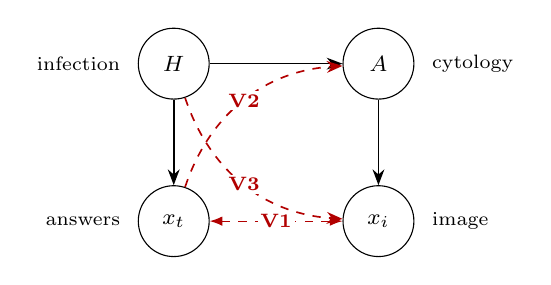
\begin{tikzpicture}[x=26mm, y=20mm, >={Latex[length=1.6mm]}]
  % latent states on the top row, observations below
  \node[var] (H)  at (0,1) {$H$};
  \node[var] (A)  at (1,1) {$A$};
  \node[var] (xt) at (0,0) {$x_t$};
  \node[var] (xi) at (1,0) {$x_i$};
  \node[font=\scriptsize, left=1mm of H]  {infection};
  \node[font=\scriptsize, right=1mm of A] {cytology};
  \node[font=\scriptsize, left=1mm of xt] {answers};
  \node[font=\scriptsize, right=1mm of xi] {image};
  % assumed structure
  \draw[arr] (H) -- (A);
  \draw[arr] (H) -- (xt);
  \draw[arr] (A) -- (xi);
  % violations, each tagged on the edge and named in the caption
  \draw[arr, dashed, red!70!black] (xt) to[bend left=34]
        node[vtag, pos=0.5] {V2} (A);
  \draw[arr, dashed, red!70!black] (H) to[bend right=34]
        node[vtag, pos=0.5] {V3} (xi);
  \draw[<->, dashed, red!70!black] (xt) -- node[vtag, pos=0.5] {V1} (xi);
\end{tikzpicture}
\caption{Assumed structure (solid) and the three violations we introduce (dashed, red). Infection $H$ drives both the questionnaire answers $x_t$ and the cytological state $A$, which in turn drives the image $x_i$; the fusion rule is exact when the dashed edges are absent. V1 is residual dependence between the two records given the latent state (strength $\rho$), V2 a direct questionnaire-to-cytology path ($\gamma$), and V3 an effect of infection on the image at fixed cytology ($\delta$). Section~\ref{sec:violations} adds each in turn.}
\label{fig:dag}
\end{figure}

\subsection{Cytology expert}
\label{sec:image}
An EfficientNet-B4 teacher \cite{tan2019efficientnet} initialised from ImageNet \cite{deng2009imagenet} is followed by global average pooling, batch normalisation, a 512-unit ReLU layer, dropout and a five-way softmax; inputs are $380\times380$ with random flips, rotations up to $\pm72^\circ$ and $\pm10\%$ zoom. Stage~1 trains the head with the backbone frozen (Adam, $10^{-3}$, up to 30 epochs, early stopping on validation loss, learning-rate reduction on plateau, class weights); stage~2 fine-tunes the whole network (Adam, $10^{-5}$, up to 50 epochs, batch size 8). An EfficientNet-B0 student is then distilled from the frozen teacher \cite{hinton2015distilling} with
\begin{equation}
\mathcal L = \alpha\,\mathrm{CE}(y,s) + (1-\alpha)\,\mathrm{KL}\!\left(\sigma(t/T)\,\|\,\sigma(s/T)\right),
\label{eq:kd}
\end{equation}
$\alpha=0.1$, $T=4$. In our implementation $t$ and $s$ are the networks' output \emph{probabilities}, so the temperature acts on probabilities rather than logits; because that is not the standard formulation we ablate it in Section~\ref{sec:imgres} against no distillation, standard logit distillation and logit distillation with the usual $T^2$ scaling.

\emph{Protocols.} \emph{A (random)}: all 5,015 images split at file level 70/20/10 (seed 42), the test set fixed as a list of 504 files. Because cropped cells and their parent fields can land on opposite sides, 404 of the 414 cropped test cells share a slide with training images. \emph{B (slide-grouped)}: the 4,049 cropped cells only, with whole source slides assigned to training, validation and test within each class (2,819/851/379 cells), so no test cell shares a slide with any training cell. Protocol~B is our primary estimate; Protocol~A is reported because it is the split used in most work on this data set.

\emph{Unit of analysis.} The expert scores a cell, whereas a deployment prevalence refers to a woman. As a step towards the coarser unit we pool the held-out cells of each source slide into a slide score (mean, maximum, mean of the top $k$, or noisy-OR) and evaluate at that level. SIPaKMeD slides carry a single class, so this is a source-image unit and not a woman with a mixed cell population; the distinction is revisited in Section~\ref{sec:limits}.

\subsection{Questionnaire expert}
\label{sec:tabular}
Six families are compared: logistic regression, $k$-nearest neighbours, random forest \cite{breiman2001random}, extremely randomised trees \cite{geurts2006extremely}, LightGBM \cite{ke2017lightgbm} and XGBoost \cite{chen2016xgboost}. Imbalance is handled by class weights rather than synthetic oversampling. Nominal items (race/ethnicity, marital status, sexual orientation) are one-hot encoded rather than left in their released integer codes; yes/no and serology items are recoded to 0/1; genuinely ordinal items keep their order; indicators are added for the 27 items with more than 5\% missing, giving 71 features. Median imputation and standardisation are fitted inside each training fold. Because choosing the best of six families on the same folds that report the score is optimistic, the family is selected by an inner five-fold cross-validation within each outer fold, and the selected pipeline is isotonically calibrated \cite{zadrozny2002transforming} in a further inner loop, so every reported probability is out of fold. Calibration is summarised by expected calibration error and by the intercept and slope of a logistic recalibration. Sensitivity analyses use the NHANES examination weights, strata and primary sampling units; a temporal split trains on 2003--2010 and tests on 2011--2016; and performance is broken out by age, race/ethnicity and cycle. Explanations use permutation importance on held-out folds, coloured by the sign of the deployed model's own coefficient.

\subsection{The fusion rule}
\label{sec:coprior}
Under label shift a posterior trained at prior $\pi$ is moved to a deployment prior $\tau$ by \cite{saerens2002adjusting}
\begin{equation}
\logit \tilde p = \logit p - \logit \pi + \logit \tau ,
\label{eq:anchor}
\end{equation}
and $\lambda=\logit p-\logit\pi$ is the evidence the input contributes, free of the prior. Re-anchoring the questionnaire to $\tau_H$ and applying the link of Section~\ref{sec:link} gives the pre-test probability of abnormal cytology,
\begin{equation}
r(x_t) = q_1\,\tilde p_H + q_0\,(1-\tilde p_H).
\label{eq:bridge}
\end{equation}
Under (A1)--(A3), $P(A\mid x_i,x_t)\propto P(x_i\mid A)P(A\mid x_t)$ and therefore
\begin{equation}
\begin{split}
\logit P(A{=}1\mid x_i,x_t) &= \lambda_i + \logit r(x_t),\\
\lambda_i &= \logit\pimg - \logit\piimg,
\end{split}
\label{eq:fuse}
\end{equation}
the questionnaire setting pre-test odds and the image multiplying them by its likelihood ratio. With only an image the output is $\sigma(\lambda_i+\logit\tau_A)$; with only a questionnaire it is $r(x_t)$; with neither it is $\tau_A$. Optionally the fused probability is floored at the re-anchored image probability when the latter exceeds $0.5$, so a low questionnaire risk cannot mask a confident abnormal read. Abstention uses Mondrian split-conformal prediction \cite{vovk2005algorithmic,angelopoulos2023conformal}: with non-conformity $1-\hat P(c)$ and class-wise thresholds at the $\lceil(n_c+1)(1-\alpha)\rceil$-th smallest calibration score, the system reports a class when the prediction set is a singleton and defers otherwise.

\subsection{Semi-synthetic paired cohorts}
\label{sec:synthetic}
Because no woman has both inputs, the fused system is scored on synthetic women assembled from real held-out records (Fig.~\ref{fig:synth}): draw $H\sim\mathrm{Bernoulli}(\tau_H)$ and $A\mid H\sim\mathrm{Bernoulli}(q_H)$, then attach a real NHANES participant with the same infection status, carrying her out-of-fold questionnaire probability, and a real held-out cell with the same abnormality status, carrying its image probability. Conditional on $(H,A)$ the two records are drawn independently, which is assumption (A1)--(A2) by construction; that is precisely why the violations below are necessary.

\begin{figure}[t]
\centering
{%
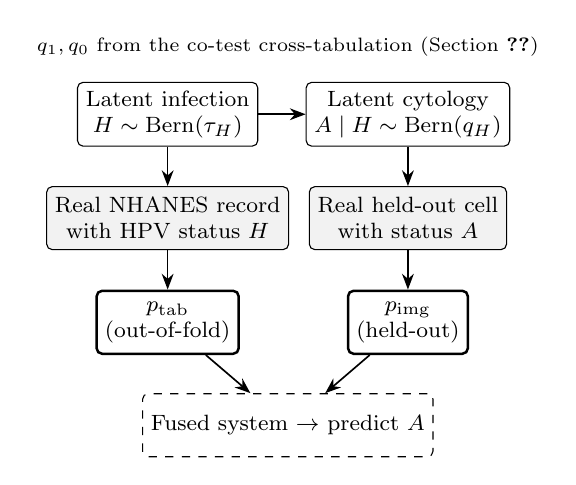
\begin{tikzpicture}[node distance=5mm and 6mm]
  \node[box] (h) {Latent infection\\$H\sim\mathrm{Bern}(\tau_H)$};
  \node[box, right=of h] (a) {Latent cytology\\$A\mid H\sim\mathrm{Bern}(q_H)$};
  \node[data, below=of h] (nt) {Real NHANES record\\with HPV status $H$};
  \node[data, below=of a] (ni) {Real held-out cell\\with status $A$};
  \node[model, below=of nt] (et) {$\ptab$\\(out-of-fold)};
  \node[model, below=of ni] (ei) {$\pimg$\\(held-out)};
  \node[op, below=9mm of $(et)!0.5!(ei)$] (f) {Fused system $\rightarrow$ predict $A$};
  \draw[arr] (h) -- (a); \draw[arr] (h) -- (nt); \draw[arr] (a) -- (ni);
  \draw[arr] (nt) -- (et); \draw[arr] (ni) -- (ei); \draw[arr] (et) -- (f); \draw[arr] (ei) -- (f);
  \node[font=\scriptsize, align=center, above=2mm of $(h.north)!0.5!(a.north)$] {$q_1,q_0$ from the co-test cross-tabulation (Section~\ref{sec:link})};
\end{tikzpicture}}
\caption{Construction of a semi-synthetic woman. Latent states are drawn from cohort-matched margins and each state selects a real held-out record. The fused system is scored on the latent cytology label.}
\label{fig:synth}
\end{figure}

\emph{Image experts.} Three are used: the Protocol~B student (in-distribution AUROC 0.995); the same network applied to Herlev with no retraining (0.641), a genuinely weak and miscalibrated expert; and, to interpolate, the Protocol~B student with Gaussian noise added to its log-odds and Platt rescaling \cite{platt1999probabilistic} on image-only data, tuned to target AUROCs of 0.95, 0.90 and 0.80.

\emph{Comparators.} The raw image output; the re-anchored image; the questionnaire pre-test risk; the naive mean and naive product of the raw outputs; the sum rule \cite{kittler1998combining} on re-anchored and bridged probabilities; \eqref{eq:fuse} with and without the safety floor; and a \emph{paired-data oracle}, a logistic stacker on $(\logit\pimg,\logit\ptab)$ refitted on paired synthetic data, which is an upper bound requiring data that do not exist in practice.

\subsection{Breaking the assumptions}
\label{sec:violations}
Six controlled violations are applied to the generator, each with the fusion unchanged and the oracle refitted so that it can exploit whatever structure appears: (V1) residual dependence between the two records given the latent state, induced by a Gaussian copula of correlation $\rho$ over the ranks from which the records are drawn, so the marginals are preserved; (V2) a direct questionnaire-to-cytology path of strength $\gamma$, violating (A2); (V3) an infection-dependent shift $\delta$ of the image score at fixed cytology, violating (A1); (V4) subgroup-varying links, with $q_1,q_0$ differing between two halves of the population while the fusion uses pooled values; (V5) unknown miscalibration of either expert, a temperature on its log-odds; and (V6) image domain shift, a bias on the image log-odds, alone and together with a prevalence change, which is label shift plus covariate shift and so steps outside (A3).

%% =====================================================================
\section{Experimental Setup}
\label{sec:setup}

\subsection{What is evaluated on what}
Nothing is evaluated on data used to fit it. The cytology expert is scored on a fixed 504-image test set (Protocol~A), on 379 cells from unseen slides (Protocol~B), and on Herlev. The questionnaire expert is scored only through out-of-fold predictions, with imputation, scaling, family selection and calibration all refitted inside folds. The fusion consumes these held-out outputs; no expert is retrained inside the fusion experiments, and the rule itself has no fitted parameters.

\subsection{Experiments}
Table~\ref{tab:experiments} lists the experiments. The synthetic ones use 20 replicates of 20,000 women; within a replicate every rule sees the same women and the same expert outputs, so differences isolate the rule. Because that comparison is paired, gains are reported as the mean and 95\% interval of the per-replicate difference, not as the difference of two independently summarised means. Uncertainty in the image expert itself is propagated by resampling its test cells between replicates.

\begin{table}[t]
\caption{Experiments and Where They Appear}
\label{tab:experiments}
\centering\footnotesize
\setlength{\tabcolsep}{3pt}
\begin{tabular}{@{}>{\raggedright\arraybackslash}p{0.05\columnwidth}>{\raggedright\arraybackslash}p{0.42\columnwidth}>{\raggedright\arraybackslash}p{0.20\columnwidth}>{\raggedright\arraybackslash}p{0.21\columnwidth}@{}}
\toprule
\# & Question and execution & Varied & Reported in \\
\midrule
1 & Cytology accuracy; one run per protocol, plus 3 seeds and a distillation ablation & Protocol A/B, seed, KD variant & Tables~\ref{tab:image}--\ref{tab:imgprot} \\
2 & External validity; same networks applied to Herlev, no retraining & Protocol A vs B & Fig.~\ref{fig:external} \\
3 & Questionnaire accuracy; 5-fold CV, in-fold preprocessing, nested family selection & Six families; weighting; era; subgroup & Table~\ref{tab:tabular}, Figs.~\ref{fig:subgroups}--\ref{fig:tabimp} \\
4 & Calibration under prevalence shift; held-out predictions resampled to a target prevalence & $\tau$; with/without re-anchoring & Fig.~\ref{fig:coprior} \\
5 & Fusion quality on matched cohorts & Link strength $\times$ image quality & Table~\ref{tab:fusion}, Fig.~\ref{fig:gain} \\
6 & Assumption violations V1--V6 & $\rho,\gamma,\delta$, subgroup, miscalibration, domain shift & Table~\ref{tab:violations}, Fig.~\ref{fig:robust} \\
7 & Price in paired data; stacker trained on $n$ paired patients & $n=50\ldots20{,}000$ & Fig.~\ref{fig:pairedneed} \\
8 & Missing inputs and abstention & Fraction missing; $\alpha$; shift & Fig.~\ref{fig:missing} \\
\bottomrule
\end{tabular}
\end{table}

\subsection{Metrics and implementation}
Image metrics are accuracy, balanced accuracy, macro-F1, Cohen's $\kappa$, macro one-versus-rest AUROC, expected calibration error (ECE) \cite{guo2017calibration} and Brier score, with sensitivity and specificity for the binary collapse. Questionnaire and fusion metrics are AUROC, average precision, Brier score, ECE, calibration intercept and slope, sensitivity at 90\% specificity, and net benefit \cite{vickers2006decision}; because the fusion cohorts are semi-synthetic, net benefit there is a simulation result and not evidence of clinical utility. Intervals are percentile bootstrap intervals over 1,000 resamples \cite{efron1994bootstrap}. Everything ran on one NVIDIA RTX 5060 Ti (16~GB) with TensorFlow 2.21 and scikit-learn 1.8 \cite{pedregosa2011scikit}; the slide-grouped teacher and student take 49 minutes, the questionnaire study under two minutes, and the fusion experiments under two minutes.

%% =====================================================================
\section{Results}

\subsection{Cytology expert}
\label{sec:imgres}
On the fixed Protocol~A test set (Table~\ref{tab:image}) the distilled student reached 96.4\% accuracy (95\% CI 94.6--98.0) and macro AUROC 0.998, matching the teacher (96.0\%, 0.996) with 4.0 times fewer parameters, an 11.4-times smaller file and 2.4 times the throughput; the difference between the two is within the confidence intervals, so the student matches rather than beats its teacher. Both are well calibrated in distribution (ECE 0.020 and 0.024). Errors concentrate between the two abnormal classes and between metaplastic and abnormal cells (Fig.~\ref{fig:imgconf}), a pattern that sends borderline cells for review rather than missing them. Grad-CAM maps \cite{selvaraju2017gradcam}, computed on the pre-softmax class score because the gradients of a saturated softmax vanish, concentrate on nuclei and perinuclear cytoplasm; at a $12\times12$ resolution they are a plausibility check rather than evidence of what the network uses, and they are reported in the supplement.
\begin{figure*}[t]
\centering
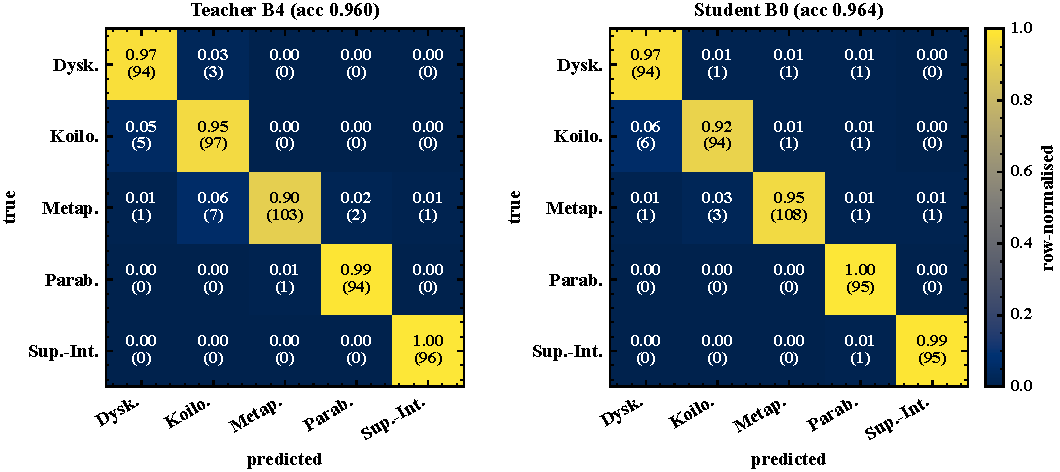
\includegraphics[width=\textwidth]{img_confusion}
\caption{Confusion matrices on the fixed Protocol~A test set, row-normalised. Both networks confuse the two abnormal classes with each other and occasionally read a metaplastic cell as abnormal; almost no abnormal cell is read as normal, which is the direction of error a screening service can tolerate.}
\label{fig:imgconf}
\end{figure*}


\begin{table}[t]
\caption{Cytology Expert, Protocol A Fixed Test Set ($n=504$)}
\label{tab:image}
\centering\footnotesize
\setlength{\tabcolsep}{4pt}
\resizebox{\columnwidth}{!}{%
\begin{tabular}{@{}lcc@{}}
\toprule
Metric & Teacher B4 & Student B0 \\
\midrule
Accuracy (95\% CI) & 0.960 (0.942--0.976) & 0.964 (0.946--0.980) \\
Balanced accuracy / macro-F1 & 0.963 / 0.961 & 0.966 / 0.965 \\
Cohen's $\kappa$ & 0.950 & 0.955 \\
Macro AUROC (95\% CI) & 0.996 (0.992--0.998) & 0.998 (0.997--0.999) \\
ECE / Brier & 0.024 / 0.065 & 0.020 / 0.057 \\
Abnormal vs normal AUROC & 0.997 & 0.999 \\
Parameters / file size & 18.6 M / 224 MB & 4.7 M / 19.6 MB \\
Latency / throughput & 141.5 ms / 138 s$^{-1}$ & 73.0 ms / 334 s$^{-1}$ \\
\multicolumn{3}{@{}l}{Both checkpoints are float32 in the same format; the teacher file}\\
\multicolumn{3}{@{}l}{also stores Adam state, so it is larger than the parameter ratio implies.}\\
\end{tabular}}
\end{table}

\emph{Slide overlap and repeats.} Under Protocol~A, 404 of 414 cropped test cells share a slide with training images, so we repeated the whole recipe with slides held out (Table~\ref{tab:imgprot}). Accuracy remained high: teacher 0.974 (0.955--0.989), student 0.958 (0.937--0.976), abnormal-versus-normal AUROC 0.995. Overlap therefore did not inflate the headline accuracy. The more useful measurement is how much a single run can be trusted at all: three independent slide-grouped runs, each redrawing the slide partition, give student accuracy \SeedStudent{} and teacher accuracy \SeedTeacher{}. That spread is an order of magnitude larger than the gap between the two protocols, so the protocol comparison -- and the teacher-versus-student comparison with it -- is dominated by which slides happen to fall in the test set, not by the design being varied. We therefore make no claim that either protocol or either network is better than the other. Aggregating the held-out cells of each of the 97 test slides gives a slide-level AUROC of 0.999 with an abnormal-slide prior of 0.474 against a cell-level prior of 0.401; since SIPaKMeD slides carry a single class, this changes the unit but not the difficulty.

\emph{Distillation ablation.} Because \eqref{eq:kd} applies the temperature to probabilities rather than logits, we compared four students under the slide-grouped protocol at a fixed seed: no distillation at all (\KDnone{}), the formulation used here (\KDprob{}), standard logit distillation (\KDlogit{}) and logit distillation with the usual $T^2$ scaling (\KDlogitTT{}). The four span one percentage point, which is well inside the $\pm0.016$ run-to-run spread above, and the undistilled student sits in the middle of the range. The honest reading is that on this data set the EfficientNet-B0 architecture, not the distillation signal, accounts for the student's performance; our nonstandard temperature placement is therefore a defect in the description rather than a source of the result, and we do not claim a distillation benefit.

\begin{table}[t]
\caption{Cytology Expert Across Protocols and Data Sets (Student)}
\label{tab:imgprot}
\centering\footnotesize
\setlength{\tabcolsep}{3.5pt}
\resizebox{\columnwidth}{!}{%
\begin{tabular}{@{}lccccc@{}}
\toprule
Setting & $n$ & Acc. & Abn. AUROC & Sens. & ECE \\
\midrule
A: random split & 504 & 0.964 & 0.999 & 0.980 & 0.020 \\
B: slide-grouped & 379 & 0.958 & 0.995 & 0.954 & 0.026 \\
B: slide level & 97 & --- & 0.999 & --- & --- \\
External (Herlev), A & 917 & 0.567 & 0.676 & 0.514 & 0.350 \\
External (Herlev), B & 917 & 0.684 & 0.641 & 0.750 & 0.247 \\
\quad excluding columnar cells & 819 & --- & 0.805 & --- & --- \\
\bottomrule
\end{tabular}}
\end{table}

\emph{External validation.} Applied unchanged to Herlev, the same student fell from 0.995 to 0.641 AUROC (95\% CI 0.595--0.684) with ECE 0.247 (Fig.~\ref{fig:external}). The failure is specific rather than diffuse: normal columnar cells, a type absent from SIPaKMeD, receive a median abnormal score of 0.979, whereas other normal cells receive 0.038 and abnormal cells 0.926. Excluding columnar cells raises external AUROC to 0.805. In-distribution accuracy on this data set therefore says little about behaviour on unseen cell types, and the weak-image regime studied below is not hypothetical: it is what this expert actually does elsewhere.

\begin{figure*}[t]
\centering
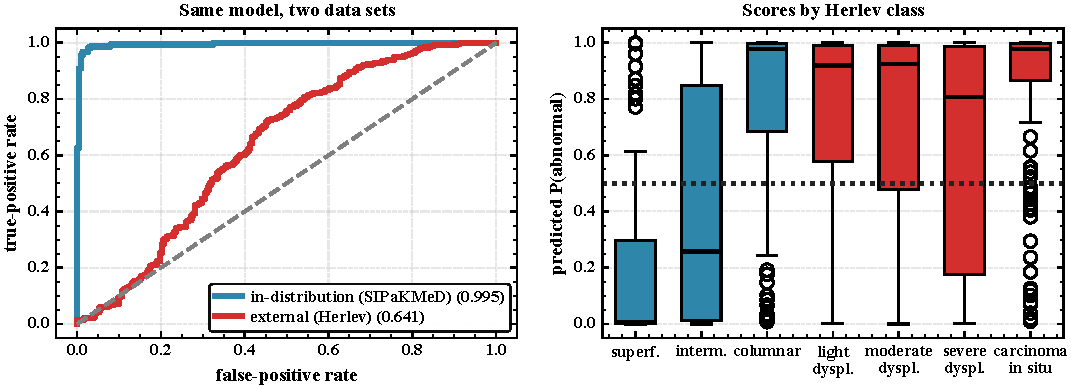
\includegraphics[width=\textwidth]{img_external}
\caption{External validation. Left: the same slide-grouped student on its own test set and on Herlev. Right: predicted abnormality by Herlev class; blue classes are normal. Columnar cells, a type never seen in training, are scored as abnormal.}
\label{fig:external}
\end{figure*}

\subsection{Questionnaire expert}
All tree ensembles and logistic regression lie between 0.663 and 0.697 AUROC with overlapping intervals, and $k$-nearest neighbours is clearly worse (0.615); with proper encoding of nominal items and missingness indicators, logistic regression is highest (0.697). Nested selection chose logistic regression in all five outer folds and gives an unbiased calibrated estimate of 0.694 AUROC with ECE 0.022 and calibration slope 1.16 (Table~\ref{tab:tabular}, Fig.~\ref{fig:tabcal}). Applying the survey design raises the estimate to 0.713 and lowers the prevalence from 24.6\% to a population-representative 22.1\%, so the unweighted analysis is, if anything, conservative. Training on 2003--2010 and testing on 2011--2016 costs little discrimination (0.684) but triples the calibration error (0.064) as prevalence drifts from 26.7\% to 21.9\% -- prior drift of exactly the kind the fusion's re-anchoring is designed to absorb. Across age, race/ethnicity and cycle, subgroup AUROC ranges from 0.637 to 0.725 and subgroup ECE stays at or below 0.050, with the largest miscalibration in the youngest women (Fig.~\ref{fig:subgroups}).
\begin{figure*}[t]
\centering
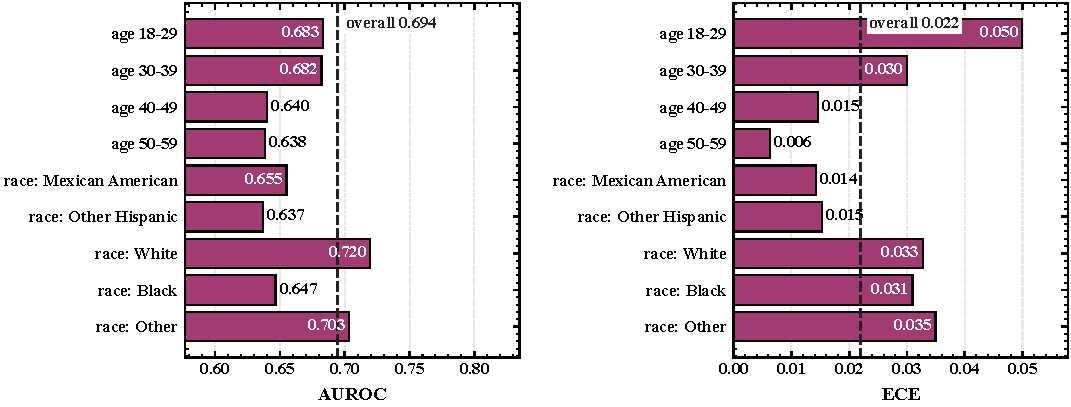
\includegraphics[width=\textwidth]{tab_subgroups}
\caption{Subgroup performance of the questionnaire expert. Discrimination (left) varies by 0.09 AUROC across age and race/ethnicity strata, and calibration error (right) stays at or below 0.050, with the largest miscalibration in women aged 18--24 -- the group in which infection is most common and most often transient.}
\label{fig:subgroups}
\end{figure*}


\begin{table}[t]
\caption{Questionnaire Expert on NHANES ($n=12{,}634$, 24.6\% Positive)}
\label{tab:tabular}
\centering\footnotesize
\setlength{\tabcolsep}{4pt}
\resizebox{\columnwidth}{!}{%
\begin{tabular}{@{}lcccc@{}}
\toprule
Analysis & AUROC & ECE & Slope & Note \\
\midrule
Logistic regression & 0.697 & 0.222 & --- & class-weighted, raw \\
LightGBM & 0.688 & 0.132 & --- & \\
Random forest & 0.686 & 0.026 & --- & \\
XGBoost & 0.686 & 0.141 & --- & \\
Extra trees & 0.663 & 0.059 & --- & \\
$k$-nearest neighbours & 0.615 & 0.120 & --- & \\
\midrule
Nested selection + isotonic & 0.694 & 0.022 & 1.16 & unbiased estimate \\
\quad survey-weighted & 0.713 & --- & --- & prevalence 0.221 \\
\quad temporal (2011--2016) & 0.684 & 0.064 & --- & prevalence 0.267$\to$0.219 \\
\quad subgroup range & 0.637--0.725 & $\leq$0.050 & --- & age, race, cycle \\
\bottomrule
\end{tabular}}
\end{table}

A permutation ranking of all 71 inputs is headed not by any answer but by the missingness flags: permuting whether the gonorrhoea question was asked costs 0.091 AUROC, and four more flags follow before the first substantive item. That ordering is an artefact rather than a finding. The flags are near-collinear, because all of them are driven by survey cycle, and the fitted model carries large offsetting coefficients on them ($+1.10$, $-0.60$, $-0.52$, $-0.49$), so permuting one destroys a cancellation the others depend on. The honest test is to remove them all, which costs 0.004 AUROC ($0.697\to0.693$); survey cycle on its own reaches only 0.539. The flags therefore inflate a sensitivity measure without carrying the signal, and we exclude them from Fig.~\ref{fig:tabimp}.

Among the answers themselves the drivers are behavioural and demographic (Fig.~\ref{fig:tabimp}): smoking status costs 0.031 AUROC, partner-acquisition rate 0.023 and ever having had oral sex 0.020, followed by marital-status contrasts and age. Directions match HPV epidemiology -- acquiring partners faster, being sexually active and younger age all raise predicted risk. Two cautions belong with the figure: the two smoking items are collinear, so their individual signs are unstable; and these are correlational markers of exposure, several of them socially sensitive, not causes of infection.
\begin{figure}[t]
\centering
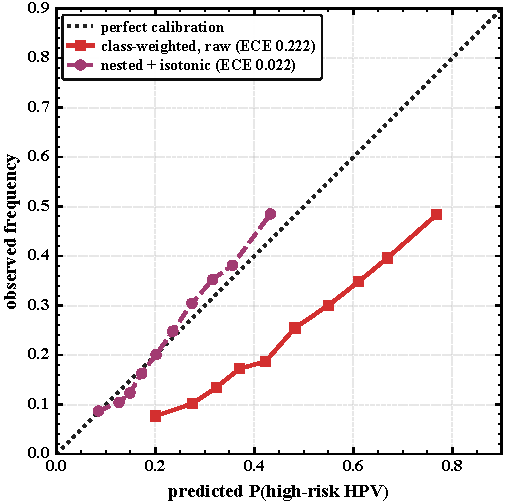
\includegraphics[width=\columnwidth]{tab_calibration}
\caption{Reliability of the questionnaire expert on out-of-fold predictions, before and after calibration. The calibrated model tracks observed frequency across the range in which it operates (ECE 0.022, slope 1.16); the raw class-weighted fit is systematically over-confident, because class weighting distorts the intercept. A weak but honest pre-test signal is what the fusion rule requires of this expert.}
\label{fig:tabcal}
\end{figure}

\begin{figure}[t]
\centering
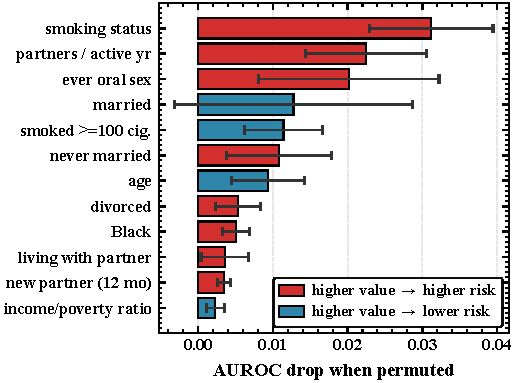
\includegraphics[width=\columnwidth]{tab_importance}
\caption{Permutation importance of the substantive questionnaire items on held-out folds, coloured by the sign of the deployed model's coefficient. Bars give the loss in AUROC when a feature is permuted. The 27 missingness flags are excluded: they are collinear and carry offsetting coefficients, so they dominate a naive ranking although removing all of them costs only 0.004 AUROC. The two smoking items are likewise collinear, so their individual directions are unstable; all items are correlational exposure markers, not causes of infection.}
\label{fig:tabimp}
\end{figure}


\subsection{Fusion}
\label{sec:fusres}

\emph{Prevalence shift on real data.} Without correction the questionnaire expert's ECE rises from 0.011 at its training prevalence to 0.111 at 12.6\% and 0.209 at 2\%; re-anchoring holds it at or below 0.011 across 2--50\% (Fig.~\ref{fig:coprior}). The sharper image expert degrades less and is likewise corrected. This is calibration under \emph{prior-probability} shift only, a distinction that matters for the domain-shift results below.
\begin{figure*}[t]
\centering
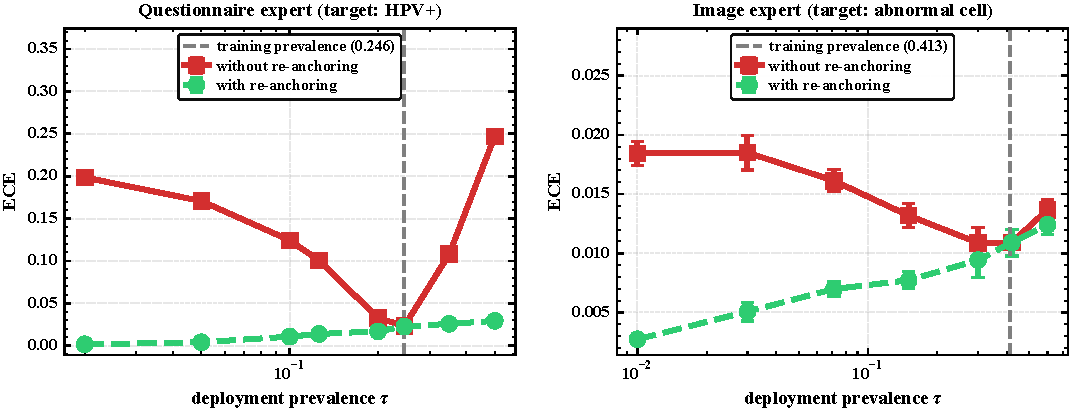
\includegraphics[width=\textwidth]{fus_coprior_real}
\caption{Calibration under prior-probability shift, computed on real held-out predictions resampled to each target prevalence. Without correction, expected calibration error grows as the deployment prevalence departs from the training prevalence (dashed vertical lines); re-anchoring with \eqref{eq:anchor} holds it near zero for both experts. This corrects the prior only, not the covariate shift studied in Fig.~\ref{fig:robust}.}
\label{fig:coprior}
\end{figure*}


\emph{When the assumptions hold.} On matched cohorts the rule behaves as the theory predicts (Table~\ref{tab:fusion}). With a near-perfect image expert nothing can improve the ranking. As image evidence weakens the questionnaire contributes more, and the gain grows with the strength of the link: for an image AUROC of 0.90 the paired gain over image-only is $+0.0027$ (95\% CI $+0.0018$ to $+0.0034$; positive in 20 of 20 replicates) at an odds ratio of 10, rising with stronger links (Fig.~\ref{fig:gain}). Across all 56 matched configurations the rule stayed within 0.0003 AUROC of the paired-data oracle and never fell below image-only by more than $10^{-5}$. Propagating uncertainty in the image expert itself by resampling its test cells widens the absolute figures considerably ($0.9048\pm0.0133$) while leaving the paired gain stable ($+0.0023\pm0.0006$), i.e.\ which expert you have matters far more than how you fuse it.
\begin{figure*}[t]
\centering
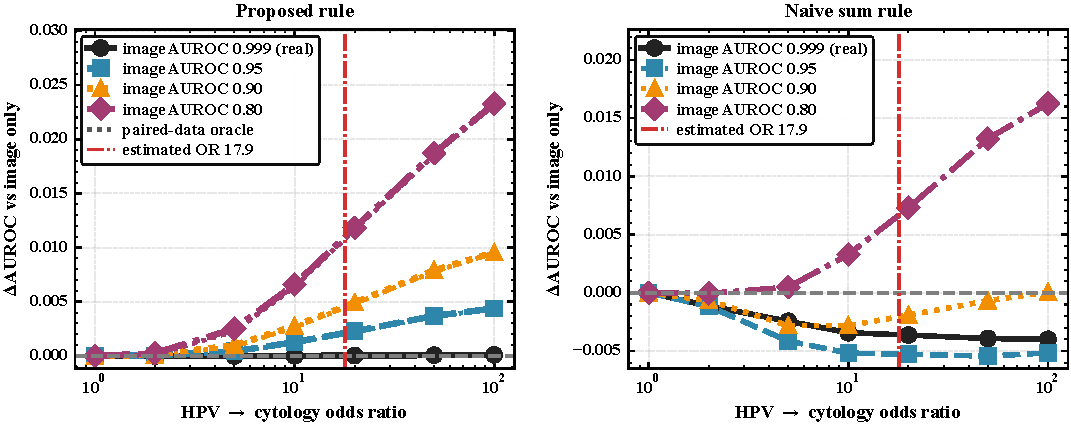
\includegraphics[width=\textwidth]{fus_gain_vs_or}
\caption{Where fusion pays, on matched cohorts. Both panels show the change in AUROC relative to the image alone as the infection--cytology link strengthens, for image experts of four qualities; dotted lines in the left panel are the paired-data oracle. The proposed rule (left) tracks the oracle and never falls below zero, whereas the naive sum rule (right) can lose ground. The benefit is largest when the image expert is weak and the link is strong; with a near-perfect image expert there is nothing left to add. The dash-dotted vertical line marks the odds ratio of 17.9 estimated in Section~\ref{sec:link}.}
\label{fig:gain}
\end{figure*}


\begin{table}[t]
\caption{Fusion on Matched and Externally Shifted Cohorts (Mean of 20 Replicates)}
\label{tab:fusion}
\centering\footnotesize
\setlength{\tabcolsep}{3pt}
\resizebox{\columnwidth}{!}{%
\begin{tabular}{@{}lcccc@{}}
\toprule
& \multicolumn{2}{c}{Matched, image 0.90} & \multicolumn{2}{c}{External image (Herlev)} \\
\cmidrule(lr){2-3}\cmidrule(l){4-5}
Method & AUROC & ECE & AUROC & ECE \\
\midrule
Image, raw & 0.8988 & 0.172 & 0.6401 & 0.446 \\
Image, re-anchored & 0.8988 & 0.004 & 0.6401 & 0.316 \\
Questionnaire, pre-test & 0.5811 & 0.003 & 0.5835 & 0.002 \\
Naive mean & 0.8949 & 0.165 & \textbf{0.6695} & 0.297 \\
Naive product & 0.8976 & 0.056 & 0.6491 & 0.365 \\
Sum rule & 0.8967 & 0.040 & 0.6412 & 0.146 \\
Proposed rule & \textbf{0.9015} & \textbf{0.003} & 0.6440 & 0.312 \\
Paired-data oracle$^{\ast}$ & 0.9014 & 0.004 & 0.6634 & 0.007 \\
\bottomrule
\multicolumn{5}{@{}l}{$^{\ast}$Requires paired training data; reference only.}
\end{tabular}}
\end{table}

\emph{When they fail.} Table~\ref{tab:violations} and Fig.~\ref{fig:robust} give the region of validity. The rule is insensitive to subgroup-varying links, to an infection-dependent image shift and to unknown miscalibration of the questionnaire, and it degrades gracefully when the link itself is misspecified by a factor of ten in either direction. Two violations matter. Residual dependence between the modalities given the latent state removes the benefit quickly: by $\rho\approx0.2$ the rule is already below image-only, and at $\rho=0.6$ it reaches 0.885 while an oracle that can learn the dependence reaches 0.922. A direct questionnaire-to-cytology path is the one violation that makes the questionnaire more informative than the rule assumes, and there naive averaging, which is not bound to the assumed structure, does better (0.9196 against 0.9082 at $\gamma=1$). And domain shift, which is covariate shift rather than label shift, is outside what \eqref{eq:anchor} can repair: the fused ECE rises from 0.010 to 0.038, and to 0.058 when a prevalence change is added.

\begin{table}[t]
\caption{Region of Validity: AUROC When Each Assumption Is Violated}
\label{tab:violations}
\centering\footnotesize
\setlength{\tabcolsep}{2.5pt}
\resizebox{\columnwidth}{!}{%
\begin{tabular}{@{}lccccc@{}}
\toprule
Violation (strength) & Image & Naive & Proposed & Oracle & ECE$_{\text{prop}}$ \\
\midrule
None & 0.8947 & 0.8893 & 0.8972 & 0.8969 & 0.010 \\
V1 dependence $\rho=0.2$ & 0.8978 & 0.8816 & 0.8951 & 0.8979 & 0.010 \\
V1 dependence $\rho=0.6$ & 0.8982 & 0.8595 & 0.8847 & \textbf{0.9217} & 0.011 \\
V2 direct path $\gamma=1$ & 0.8940 & \textbf{0.9196} & 0.9082 & 0.9245 & 0.013 \\
V3 infection$\to$image $\delta=0.4$ & 0.9270 & 0.9156 & 0.9250 & 0.9267 & 0.027 \\
V4 subgroup link (spread 0.5) & 0.8937 & 0.8879 & 0.8959 & 0.8957 & 0.011 \\
V5 miscalibrated image ($T{=}2$) & 0.8947 & 0.8813 & 0.8955 & 0.8969 & 0.026 \\
V6 domain shift & 0.8947 & 0.8893 & 0.8972 & 0.8969 & 0.038 \\
V6 domain shift $+$ prevalence & 0.8934 & 0.8891 & 0.8962 & 0.8961 & 0.058 \\
\bottomrule
\multicolumn{6}{@{}l}{Oracle requires paired training data; bold marks a rule beating the proposed one.}
\end{tabular}}
\end{table}

\begin{figure*}[t]
\centering
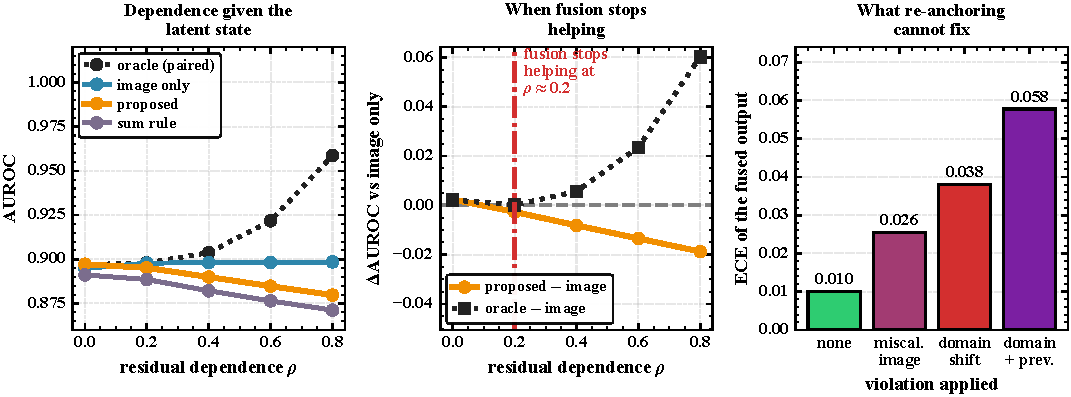
\includegraphics[width=\textwidth]{fus_robust}
\caption{Region of validity. Left: as residual dependence grows, an oracle with paired data gains while the unpaired rule loses. Centre: the gain over image-only crosses zero near $\rho=0.2$. Right: re-anchoring removes prior-shift miscalibration but not the miscalibration caused by domain shift.}
\label{fig:robust}
\end{figure*}

\emph{Under real domain shift.} With the Herlev expert the picture changes in a way worth reporting plainly (Table~\ref{tab:fusion}, right). The rule still adds a small, consistent ranking gain over image-only ($+0.0039$, 95\% CI $+0.0031$ to $+0.0046$, 20 of 20 replicates), but the naive mean does better still (0.6695), and the oracle both ranks better and is calibrated (ECE 0.007) where the unpaired rule is not (0.312). The reason is visible in the assumption analysis: a domain-shifted expert violates (A3), and a rule that trusts its probabilities inherits that error, while naive averaging dilutes it and a stacker refitted on shifted paired data simply learns around it. Principled fusion is therefore not universally better than naive fusion; it is better when its assumptions approximately hold.

\emph{The price in paired data.} On matched cohorts a logistic stacker trained on 50 paired patients is worse than the unpaired rule by 0.014 AUROC, closes to within 0.002 by 200, and never overtakes it, remaining within 0.0004 even at 20,000 (Fig.~\ref{fig:pairedneed}); that is expected, because the rule is already optimal when its assumptions hold. The unpaired rule is therefore worth roughly two hundred paired patients \emph{in the regime it was designed for}. Paired data pay off where the assumptions fail: under residual dependence of $\rho=0.6$ the oracle gains 0.037 AUROC over the rule (Table~\ref{tab:violations}), because it can learn a structure the rule is not allowed to represent.
\begin{figure}[t]
\centering
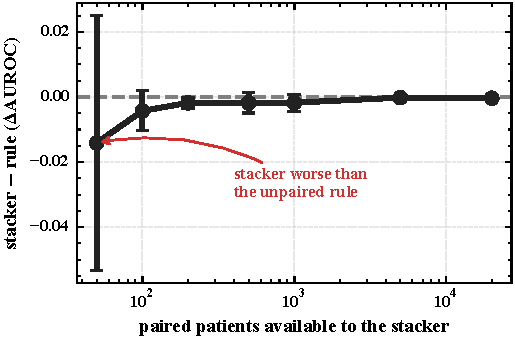
\includegraphics[width=\columnwidth]{fus_paired_need}
\caption{What the unpaired rule is worth in paired patients. A logistic stacker trained on $n$ paired women is compared with the unpaired rule, which uses none. Below about two hundred paired patients the stacker is clearly worse; beyond that the two are indistinguishable, because on matched data the unpaired rule is already optimal. Error bars are standard deviations over 20 replicates.}
\label{fig:pairedneed}
\end{figure}


\emph{Missing inputs and abstention.} The any-modality output degrades smoothly as inputs disappear (Fig.~\ref{fig:missing}): with an image AUROC of 0.90 the AUROC falls from 0.903 to 0.854, 0.784 and 0.691 as 25\%, 50\% and 75\% of women lose their image, and to 0.577 when only questionnaires remain, while removing questionnaires changes it by at most 0.002. Conformal abstention met its target on matched data (coverage 0.901 at a 0.90 target, deferring 21\% of women) but not under shift: coverage fell to 0.880 under dependence and to 0.755 under domain shift plus prevalence change, and a miscalibrated image expert held coverage only by deferring 48\% of women. Coverage guarantees are conditional on exchangeability, and domain shift breaks it.
\begin{figure}[t]
\centering
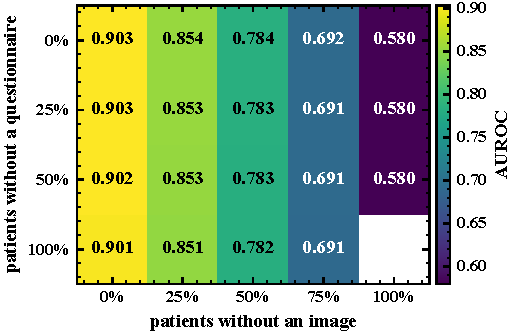
\includegraphics[width=\columnwidth]{fus_missing_090}
\caption{Any-modality behaviour. As images are withheld from a growing fraction of women the fused AUROC falls smoothly towards the questionnaire-only level rather than failing; withholding questionnaires instead costs almost nothing, because with this image expert the questionnaire contributes little ranking information.}
\label{fig:missing}
\end{figure}


%% =====================================================================
\section{Discussion}
Two experts trained on disjoint populations can be combined into one calibrated screening output without paired data, and the arithmetic for doing so is elementary once the endpoints and priors are handled explicitly. The useful result is not that the rule works, which follows from its assumptions, but where it stops working. It tolerates a link misspecified by an order of magnitude, links that vary by subgroup, an infection-dependent image shift and a miscalibrated questionnaire. It does not tolerate residual dependence between the modalities beyond about $\rho=0.2$, and it cannot repair the miscalibration that domain shift produces. Both failures are diagnosable in practice: dependence can be estimated from even a small paired sample, and domain shift is visible from score distributions without labels.

The external validation reframes the rest. A network at 0.995 AUROC in distribution falls to 0.641 on another laboratory's images, almost entirely because a cell type it never saw is confidently called abnormal; with that type removed it reaches 0.805. This is the regime in which fusion has something to add, and also the regime in which the fusion's own assumption (A3) is most doubtful -- which is why, with the Herlev expert, naive averaging beats the principled rule on ranking and the paired oracle beats both on calibration. We report that rather than tuning around it.

A second reframing concerns what the image expert is a probability \emph{of}. Re-anchoring is a statement about one random variable observed under two priors; a cell drawn from a curated collection and a woman attending a clinic are not that variable. Pooling cells to a slide moves one step towards the clinical unit and leaves discrimination untouched, but SIPaKMeD slides are single-class, so the step is smaller than it looks. Until an image expert is trained and calibrated at the level of a whole smear, the calibration results here demonstrate the operator, not patient-level risk.

For the questionnaire expert, the statistical choices mattered in the direction the design predicts but not in magnitude: one-hot encoding of nominal items and missingness indicators raised AUROC from 0.687 to 0.697, nested selection cost 0.003, and survey weighting raised it to 0.713. The model is a stable but weak pre-test signal, and the temporal experiment shows its calibration, not its ranking, is what drifts. Its strongest items -- smoking status, partner-acquisition rate, reported sexual practice and marital-status contrasts -- are social proxies rather than biological ones; they carry information because they stand in for exposure, and a service that used them would be assigning risk on the basis of relationship status and reported behaviour. We report them transparently and stratify by age and race/ethnicity rather than assume the model behaves uniformly, but deciding whether such proxies belong in a deployed screening tool is a policy question, not a modelling one.

Finally, a note on what the system predicts. The endpoint here is cytological abnormality, which is a screening test result and not disease; the clinically decisive endpoint is histologically confirmed CIN2+ \cite{wright2012athena}. The bridge in \eqref{eq:bridge} could target that endpoint directly given the corresponding rates, and the same machinery would apply, but the evidence in this paper does not extend to it.

\subsection{Limitations}
\label{sec:limits}
\begin{itemize}
\item \emph{Fusion is evaluated semi-synthetically.} No woman has both inputs. The cohorts use real held-out records and cohort-matched margins, and the violation study probes the structure, but only a prospective paired cohort can settle the question.
\item \emph{Unit of analysis.} The image expert scores a cell, or at best a single-class source image, whereas prevalence refers to a woman with thousands of mixed cells. The calibration results should be read as demonstrating the operator under prior shift, not as patient-level calibrated risk.
\item \emph{Endpoint.} Cytological abnormality is a surrogate for precancer.
\item \emph{Populations differ.} The link comes from U.S. women aged 30 and over, the questionnaire from U.S. women aged 18--59 surveyed in 2003--2016, the images from a Greek laboratory. Re-anchoring handles prevalence differences, not differences in how risk factors relate to infection.
\item \emph{External validation is single-source.} One external cytology set was used; broader validation across staining and scanners remains open.
\item \emph{Run-to-run variation exceeds the effects being compared.} Three slide-grouped runs span 0.928--0.958 for the student and 0.914--0.974 for the teacher. Nothing in this paper that rests on a difference of one or two percentage points between two image models should be read as a real difference, including the teacher-versus-student and Protocol~A-versus-B comparisons; the number of independent runs a fair comparison would need is larger than we ran.
\end{itemize}

%% =====================================================================
\section{Conclusion}
We combined a cytology classifier and an HPV-risk questionnaire model, trained on data sets sharing no patients, into a calibrated any-modality screening output, using an epidemiological link estimated from 812,598 screening co-tests rather than assumed. Where its assumptions hold the rule matches a model trained on paired patients and is worth about two hundred of them. Where they fail it does not: residual dependence beyond $\rho\approx0.2$ removes its advantage, and domain shift, which our external validation shows is the operative regime for the image expert, defeats its calibration. Mapping that boundary, rather than the fusion itself, is what we would carry forward: a prospective paired pilot large enough to estimate the residual dependence, and an image expert validated across laboratories, are the prerequisites for clinical use.

\section*{Data and Code Availability}
SIPaKMeD, Herlev and NHANES are public. The evaluation scripts, fixed test-set file lists, per-case held-out predictions, the cohort simulator with all random seeds, and the figure-generation code are released at \url{https://github.com/ORGANISATION/REPOSITORY} (DOI to be assigned on acceptance).

\section*{Acknowledgment}
The authors thank [to be completed].

\bibliographystyle{IEEEtran}
\bibliography{Mybib,refs_added}

\end{document}
